\documentclass{article} % For LaTeX2e
\usepackage{nips15submit_e,times}
\usepackage{hyperref}
\usepackage{url}
\usepackage{calrsfs}
\usepackage{graphicx}
\usepackage{float}
\usepackage{geometry}
\usepackage{qtree}
\usepackage{natbib}
\usepackage{caption}
\usepackage{subcaption}

\graphicspath{ {images/} }
\DeclareMathAlphabet{\pazocal}{OMS}{zplm}{m}{n}
\newcommand{\La}{\mathcal{N}}
\newcommand{\Lb}{\pazocal{N}}
%\documentstyle[nips14submit_09,times,art10]{article} % For LaTeX 2.09


\title{Generative Models for Image Generation}


\author{
Vishal Vijayvargiya
Mahya Sadeghi
Amineh Dadsetan
Kiana Mostaghasi
Amirmasoud Toudeshki
}


% The \author macro works with any number of authors. There are two commands
% used to separate the names and addresses of multiple authors: \And and \AND.
%
% Using \And between authors leaves it to \LaTeX{} to determine where to break
% the lines. Using \AND forces a linebreak at that point. So, if \LaTeX{}
% puts 3 of 4 authors names on the first line, and the last on the second
% line, try using \AND instead of \And before the third author name.

\newcommand{\fix}{\marginpar{FIX}}
\newcommand{\new}{\marginpar{NEW}}

%\nipsfinalcopy % Uncomment for camera-ready version

\begin{document}


\maketitle

\begin{abstract}
    This report presents two approaches for artificial image generation using generative models, namely, Variational Autoencoders (VAE) and Generative Adversarial Networks (GAN). VAEs are appealing because they are built on top of standard function approximators (neural networks), and can be trained with stochastic gradient descent. In GAN, we train two models: a generative model G that captures the data distribution, and a discriminative model D that estimates the probability that a sample came from the training data rather than G. Experiments demonstrate potential of both the approaches and an analysis is performed to study the advantages and disadvantages of them.
\end{abstract}
\section{Introduction}
Generative image algorithms are being in interest of researchers and have two main categories: parametric and non-parametric \cite{yek}. The non-parametric models mostly deal with matching from a database of existing images and have been used in texture synthesis \cite{do}, super-resolution  \cite{seh} and in-painting \cite{chahar}.

On the other hand, parametric models for image generation has been studied deeply (for example on MNIST digits or for texture synthesis \cite{panj}). However, generating natural images of real world  is still a big issue and had not been successful until recently. 
A recurrent network approach \cite{shish} and a deconvolution network approach \cite{haft}  have recently had some success with generating natural images. Another approach generates images using an iterative forward diffusion process \cite{hasht}.

A variational sampling approach to generating images \cite{noh} has had some success. In just three years, Variational Autoencoders (VAEs) have showed up as one of the most popular approaches to unsupervised learning. VAEs are appealing because they are built on top of standard function approximators (neural networks), and can be trained with stochastic gradient descent.                   

VAEs have already shown progress in generating several types of complicated data, including handwritten digits, faces, segmentation, and predicting the future from static images. 

Another well known algorithm in this area is Generative Adversarial Networks. GAN attempts to train an image generator by simultaneously training a discriminator to challenge it to improve.

(Generative Adversarial Nets) compares challenges in generative models. It mentions challenges in training, inference, sampling and model design for four generative model: deep directed graphical models,  deep undirected graphical models, generative autoencoders and adversarial models. 
In our project we try to test Variational Autoencoder (VAN) and Generative Adversarial Networks (GAN) for two data set: faces and a landscape time lapse. We want to show how this two major algorithms could generate new images based on training data of real world image. 

\section{Approaches}
We used three different approaches to generate new images from a given dataset of images. Our first approach is to use an auto-encoder that is to encode an image to a reduced set of features and then construct the image from the reduced feature set. In that way first we train an encoder neural network to encode our images and with the encoded data we train a decoder neural network that can generate pictures from a small set of features. Using this approach we construct an application that can generate a picture that is similar to two given picture from our dataset with defined percentage. Our approach to do that is to use the set of encoded features of each image and generate new set of encoded features. With the new generated encoded feature set, using the decoder part we generate the picture.

After using this approach, we were interested to implement other kinds of generative models to generate new images given a dataset of images. Those models are variational auto-encoder and generative adversarial nets. In the following sections, we are going to discuss these structures.

\subsection{Variational autoencoder(VAE)}
Variational Autoencoder is one of the methods that we used to generate new data from our given data. 

The idea is to use variational inference. In varational inference schema, instead of computing posterior distribution over the latent variable, we assume that latent variable is from a specific probability distribution function like $q_{\phi}(z)$ in which z is our latent variable and $\phi$ is the varitional parameter of the distribution that we can change through optimization. From this prior distribution and with the assumption that the posterior distribution $q_{\phi}(z|x)$ is a gaussian, we can approximate this  distribution. To do that, we set the $q_{\phi}(z|x)$ to be the out put of encoder part.
Thus, the logarithm of posterior distribution function is:
\begin{equation}
log\ q_{\phi}(z|x^{(i)}) = log \Lb(z; \mu^{(i)}, \sigma^{2(i)}I)
\end{equation}
Now to measure how how much our approximation is close to the real answer, we need to compute two things: 1- The latent loss and 2- the generation loss. The first term in computing error is to do the difference between the distribution of $q_{\phi}(z|x)$ and $q_{\phi}(z)$ which we aim to minimize it( works like a regulizer) and we can comput it with KL-divergence.  The second term is due to the different between our generated image and the main image. As we see the first term try to prevent the output to be very close to input and instead try to minimize the differenc between $q_{\phi}(z|x)$ and $q_{\phi}(z)$(which is a unit gaussian).

Now, the question is how to compute the different between our generated image and the main image while we havn't generated image yet. The answer is to sample the z from the posterior distribution function $q_{\phi}(z|x)$. To do this sampling we need a reparametrization. Assuming $z \sim q_{\phi}(z|x)$ we will have 
\begin{equation}
z = \mu + \sigma^2 \times \epsilon,\ \epsilon \sim \Lb(0, I)
\end{equation}
It means that to sample z from the mean vector and variance vector, we just need to sample $\epsilon$ from a unit guassian distribution. After sampling this function we can compute a mean squared error for the generation loss term.

Finally the structure of the network that we are using is described in Figure \ref{structure}.
\begin{figure}[h]
    \centering
    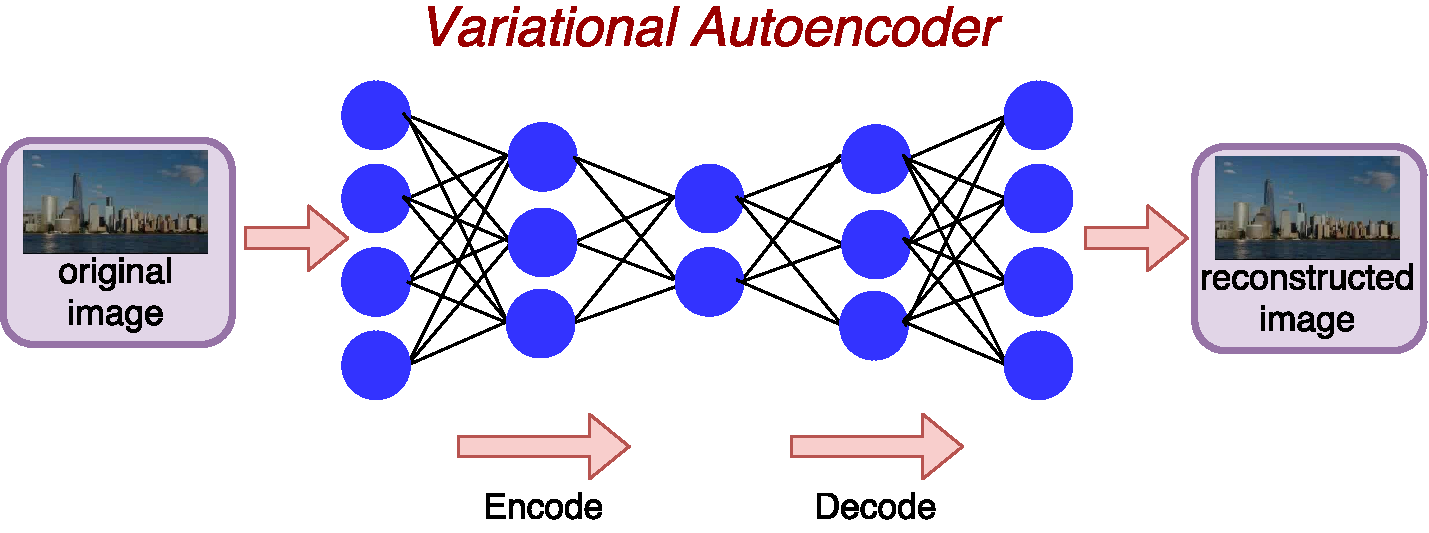
\includegraphics[width=8cm]{structure.pdf}
    \caption{Structure of neural network used in VAE.}
        \label{structure}
\end{figure}
\subsection{Generative adversarial nets}
So far, the most striking successes in deep learning have involved discriminative models, and these striking successes have primarily been based on the backpropagation and dropout algorithms, using piecewise linear units which have a particularly well-behaved gradient. Deep generative models have had less of an impact, due to the difficulty of approximating many intractable probabilistic computations that arise in maximum likelihood estimation and related strategies, and due to difficulty of leveraging
the benefits of piecewise linear units in the generative context. We used a new generative model
estimation procedure that sidesteps these difficulties.

GAN (or Generative Adversarial Nets) is a framework for estimating generative models via an adversarial process. In this framework we simultaneously train two models:  
\begin{itemize}
    \setlength\itemsep{-1em}
    \item A generative model G that captures the data distribution,
    \item A discriminative model D that estimates the probability that a sample came from the training data rather than G.
\end{itemize}
In the space of arbitrary functions G and D, a unique solution exists, with G recovering the training data distribution and D equal to 1/2 everywhere. In the case where G and D are defined by multilayer perceptrons, the entire system can be trained with back-propagation.

We consider the special case (adversarial nets) when the generative model generates samples by passing random noise through a multilayer perceptron. The discriminative model is also a multilayer perceptron. In this case, we can train both models using only the highly successful back-propagation and dropout algorithms and sample from the generative model using only forward propagation.

Figure \ref{diag} shows the structure of the network and the algorithm in figure \ref{algo} describes the algorithm.
\begin{figure}[H]
\centering
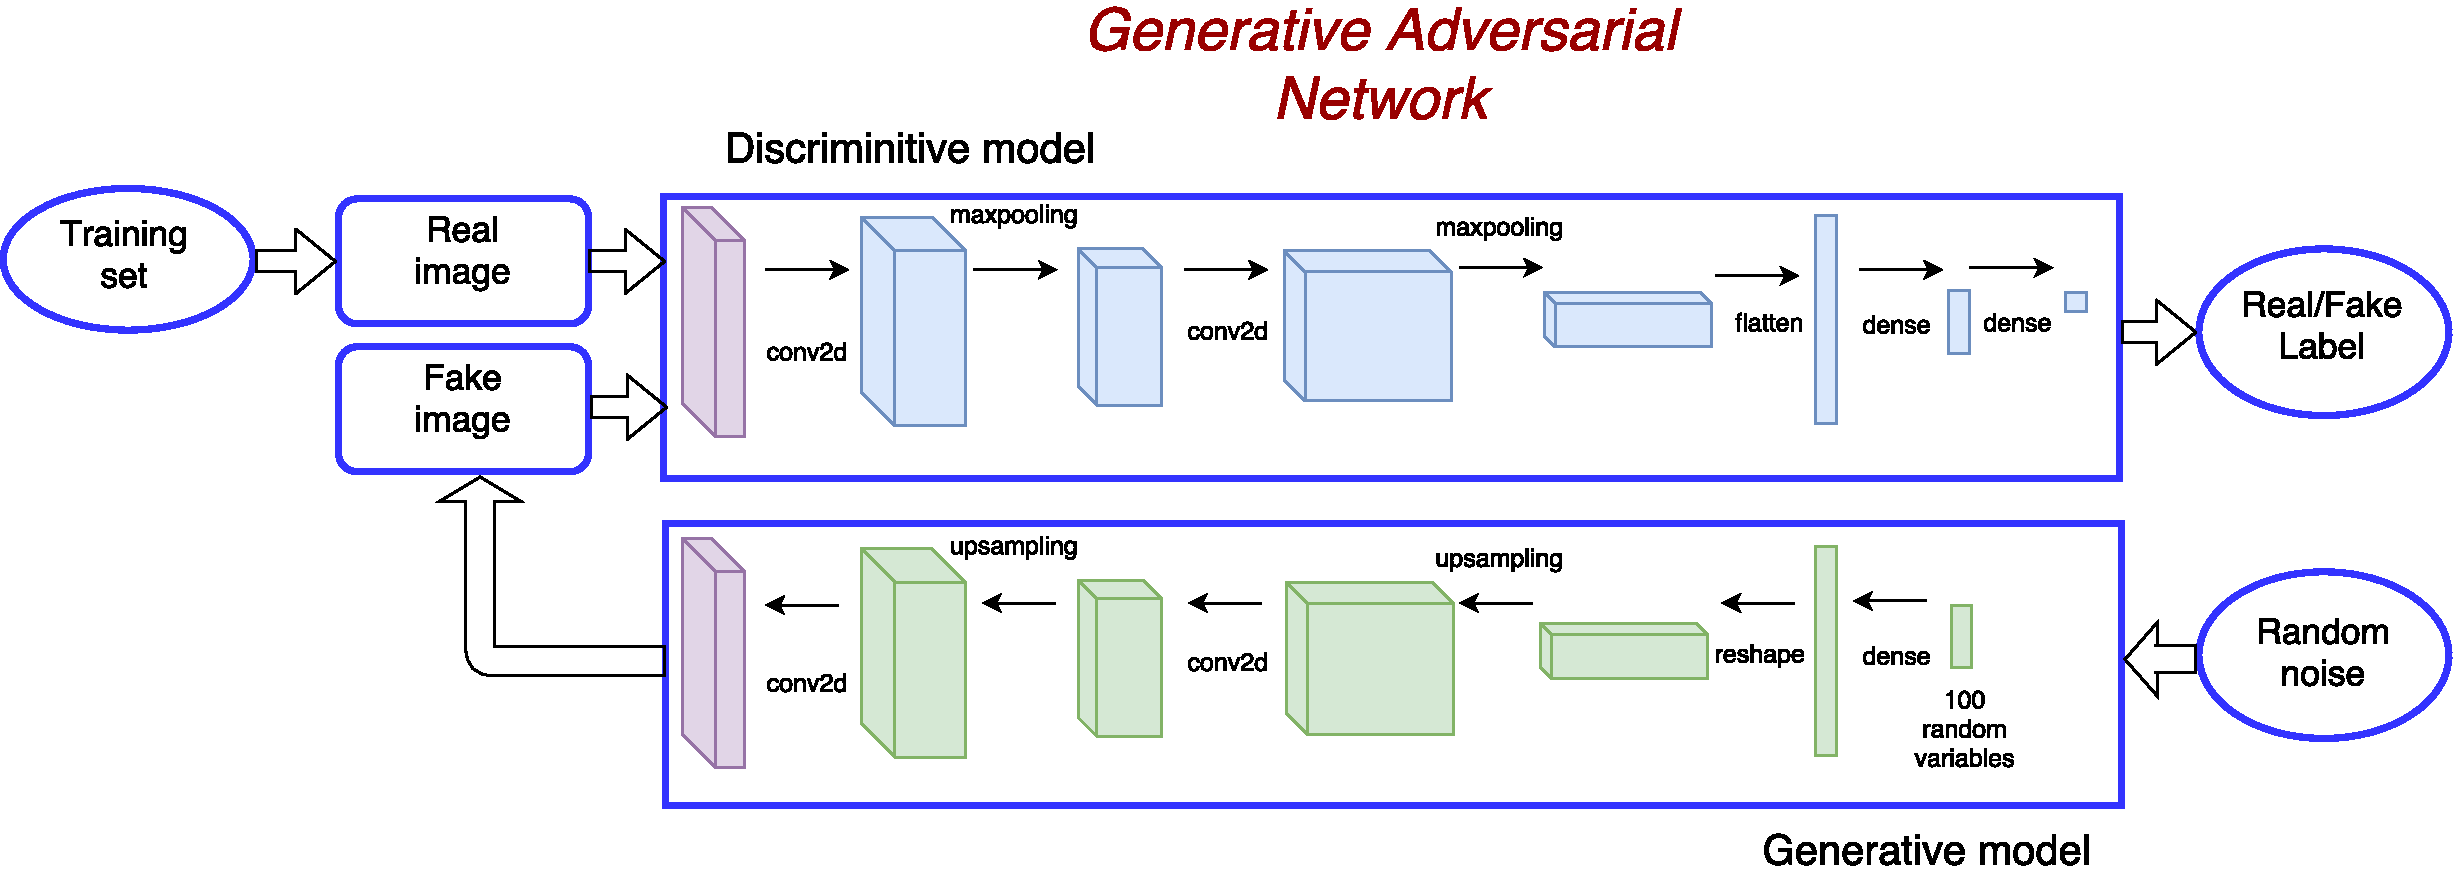
\includegraphics[width=15cm]{GAN-diagram.pdf}
\caption{Diagram for GAN}
\label{diag}
\end{figure}
\begin{figure}[h]
    \centering
    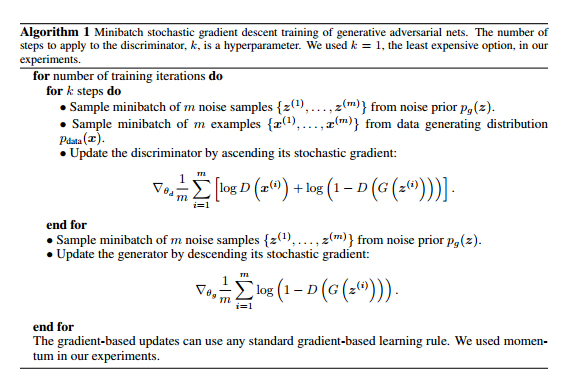
\includegraphics[width=12cm]{algo.jpg}
    \caption{GAN algorithm}
    \label{algo}
\end{figure}

\section{Experiments}
We tested our implementation of VAE and GAN on multifarious datasets. The most interesting datasets were Celebrity Face Dataset (CFD) \cite{celeb} and New York Skyline Dataset (NYSD) \cite{skyline}. CFD contained colored images of size $64 \times 64$, with training set size 9000 and test set size 1000. NYSD was created using frames of a video, partitioned into 1200 training images and 125 test images, each of size $64 \times 64$.  Our experiment setting is as follows:
\begin{itemize}
    \item    batch size = 100
    \item     original dimension = 12288 (this is 64 $\times$  64 $\times$  3i)
    \item    intermediate dimension (hidden layer nodes) = 512
    \item    latent dimension (encoded dimension) = 2
    \item    number of epoch = 250
    \item    epsilon\_std = 1.0
\end{itemize}

    Selecting a good model architecture for GAN is very crucial for faster and better results. We tried various modifications, this includes experimenting with different activation functions like ReLU and tanh, using 2-3 layers of convolution, droput layer in discriminator and batch normalization in discriminator and generator. Different combinations gave different results, finally concluding with following architecture:

    Generator Model( We are showing each layer with its dimension and its activation fucntion):

        input dimension = 100 $\rightarrow$ dense(1024) $\rightarrow$ dense(128 $\times$ 16 $\times$ 16) $\rightarrow$ 
        BatchNormalization() $\rightarrow$ Activation('tanh') $\rightarrow$ Reshape(128, 16, 16) $\rightarrow$ UpSampling2D(size=(2, 2)) $\rightarrow$
        Convolution2D(64, 5, 5, border\_mode='same') $\rightarrow$
        Activation('tanh') $\rightarrow$
        UpSampling2D(size=(2, 2)) $\rightarrow$ 
        Convolution2D(3, 5, 5, border\_mode='same') $\rightarrow$
        Activation('tanh') $\rightarrow$
        Output Image
    
Discriminator model:

        Image $\rightarrow$
 Convolution2D(64, 5, 5, border\_mode='same') $\rightarrow$
 Activation('tanh') $\rightarrow$
 MaxPooling2D(pool\_size=(2, 2)) $\rightarrow$
 Convolution2D(128, 5, 5) $\rightarrow$
 Activation('tanh') $\rightarrow$
 MaxPooling2D(pool\_size=(2, 2)) $\rightarrow$
 Flatten() $\rightarrow$
 Dense(1024) $\rightarrow$
 Activation('tanh') $\rightarrow$
 Dense(1) $\rightarrow$
 Activation('sigmoid')

\section{Results}
Figures show the results we obtained from VAE and GAN. VAE on skyline dataset generated most interesting results, with colorful sky in images. It should be noted that the original dataset didn't contain sky with red color, but VAE generated it. VAE for face dataset provided new faces but with some blur.

      For GAN the results were sharp but with some irregularities. This could be attributed to less number of epochs, as training GAN takes time. Figure also shows results obtained on various epochs.
      \subsection{Analysis and Conclusion}

    Since both the models are "generative" with completely different approach, it is difficult to come up with a common comparison criteria. We provide benefits and drawbacks of both the techniques as part of analysis.

Pros:
\begin{itemize}
\item     VAE - We can compare generated images directly to the originals, which is not possible when using a GAN
\item     VAE - Gives decent results in less training time
\item     GAN - Can generate the sharpest images
    \end{itemize}
Cons:
\begin{itemize}
\item     VAE - Network tends to produce more blurry images
\item     GAN - No way of determining which initial noise values would produce a particular picture
\item     GAN - Can lead to results where there’s no actual object in a generated image, but the style just looks like picture
    \end{itemize}
    With our project we can conclude that the problem of generating realistic-looking images is complex. Both the approaches generate good artificial images, thus providing a novel way for data augmentation and image encoding. As a future work, it is possible to get better results if we combine VAE and GAN. Using the same encoder-decoder set-up, but using an adversarial network as a metric for training the decoder.

    \begin{figure}[H]
\centering
\begin{subfigure}{.5\textwidth}
\centering
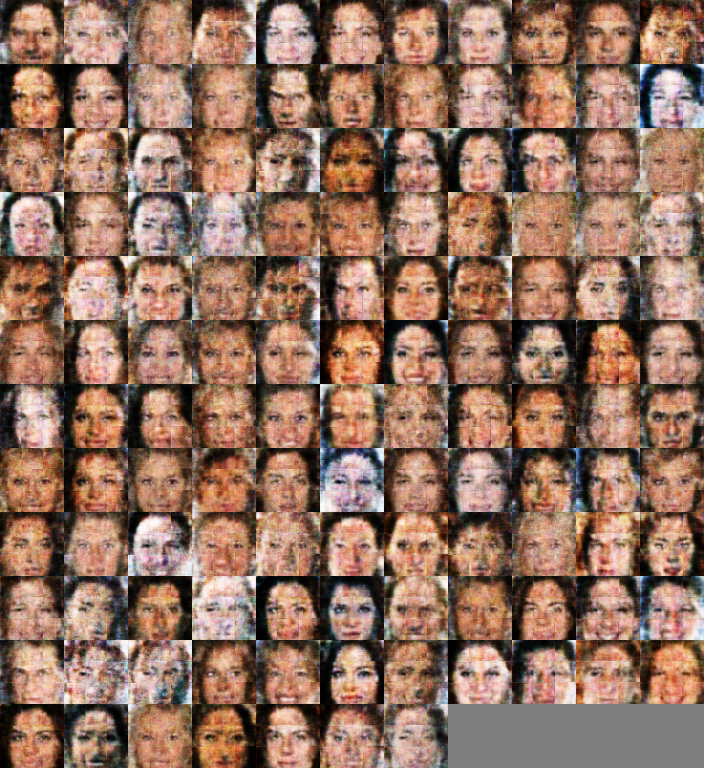
\includegraphics[width=.6\linewidth]{GAN1.png}
\end{subfigure}%
\begin{subfigure}{.5\textwidth}
\centering
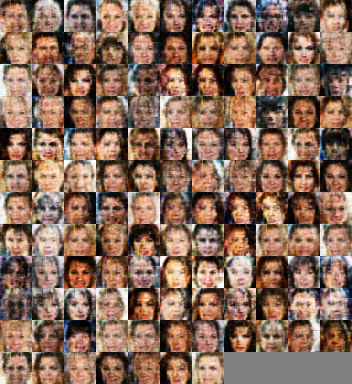
\includegraphics[width=.6\linewidth]{GAN2.png}
\end{subfigure}
\caption{Generated images with GAN}
\end{figure}

\begin{figure}[H]
\centering
\begin{subfigure}{.5\textwidth}
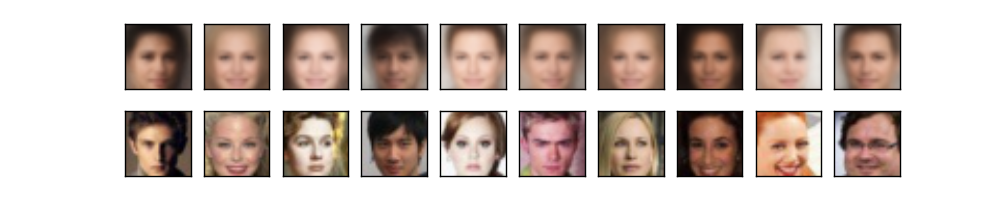
\includegraphics[width=6cm]{face_VAE.png}
\end{subfigure}%
\begin{subfigure}{.5\textwidth}
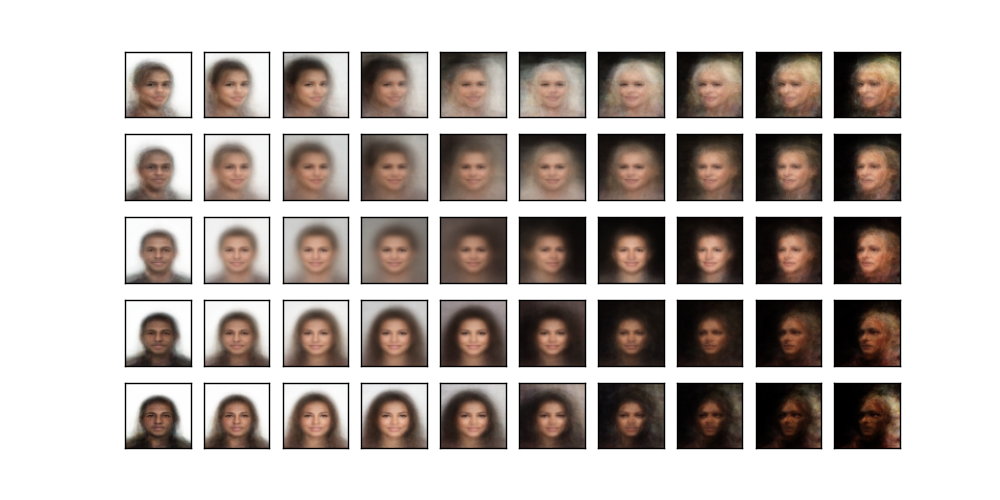
\includegraphics[width=6cm]{final_face_VAE.png}
\end{subfigure}
\caption{Generated images with VAE}

\end{figure}
\begin{figure}[H]
    \centering
    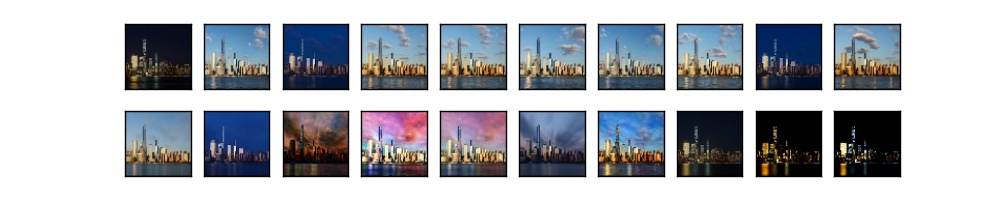
\includegraphics[width=10cm]{final_skyline_VAE.png}
    \caption{Generated Images with VAE and Skyline dataset}
    \label{skivae}
\end{figure}
\section{Contribution}
Amineh - Worked on VAE model selection and implementation and implemented simple interface\\
Vishal - Worked on GAN model selection and implementation\\
Kiana - Worked on improving traditional autoencoder and poster\\
Mahya and Amirmasoud - Worked on possible techniques to improve VAE and dataset search\\

\subsection*{Refrences}
    \renewcommand{\section}[2]{}
%\bibitem{celeb} 
%Celebrity Face Dataset - http://mmlab.ie.cuhk.edu.hk/projects/CelebA.html
%\bibitem{skyline}
%New York Skyline Video - https://www.youtube.com/watch?v=DDo73Njxdqc

\bibliographystyle{unsrt}
\bibliography{refs} 


\end{document}
